\documentclass{article}
\usepackage{amsmath, graphicx}
\begin{document}

\title{Aggregate Demand and Aggregate Supply- Solutions}
\author{ECON 101: Macroeconomics}
\date{}
\maketitle

\section*{Exercise 1: Calculating AD and AS Equilibrium}
The aggregate demand (AD) and short-run aggregate supply (SRAS) for an economy are given by the following equations:
\begin{align*}
    AD: & \quad Y = 5000 - 200P \\
    SRAS: & \quad Y = 2500 + 100P
\end{align*}
where \(Y\) is real GDP and \(P\) is the price level.

\textbf{Questions:}
\begin{enumerate}
    \item Find the equilibrium price level (\(P^*\)) and equilibrium output (\(Y^*\)).
    \item Suppose consumer confidence decreases, shifting AD to \( Y = 4800 - 200P \). Find the new equilibrium.
    \item Illustrate the initial and new equilibrium graphically using AD and AS curves.
\end{enumerate}

\textbf{Solutions:}
\begin{enumerate}
    \item To find equilibrium, set AD equal to SRAS:
    \begin{align*}
        5000 - 200P &= 2500 + 100P \\
        2500 &= 300P \\
        P^* &= \frac{2500}{300} \approx 8.33
    \end{align*}
    Substituting \(P^*\) into either equation to find \(Y^*\):
    \begin{align*}
        Y^* &= 5000 - 200(8.33) \approx 3333.33
    \end{align*}
    
    \item For the new AD equation \( Y = 4800 - 200P \), solve:
    \begin{align*}
        4800 - 200P &= 2500 + 100P \\
        2300 &= 300P \\
        P^* &= \frac{2300}{300} \approx 7.67
    \end{align*}
    \begin{align*}
        Y^* &= 4800 - 200(7.67) \approx 3266.67
    \end{align*}
\end{enumerate}


\begin{figure}[h!]
    \centering
    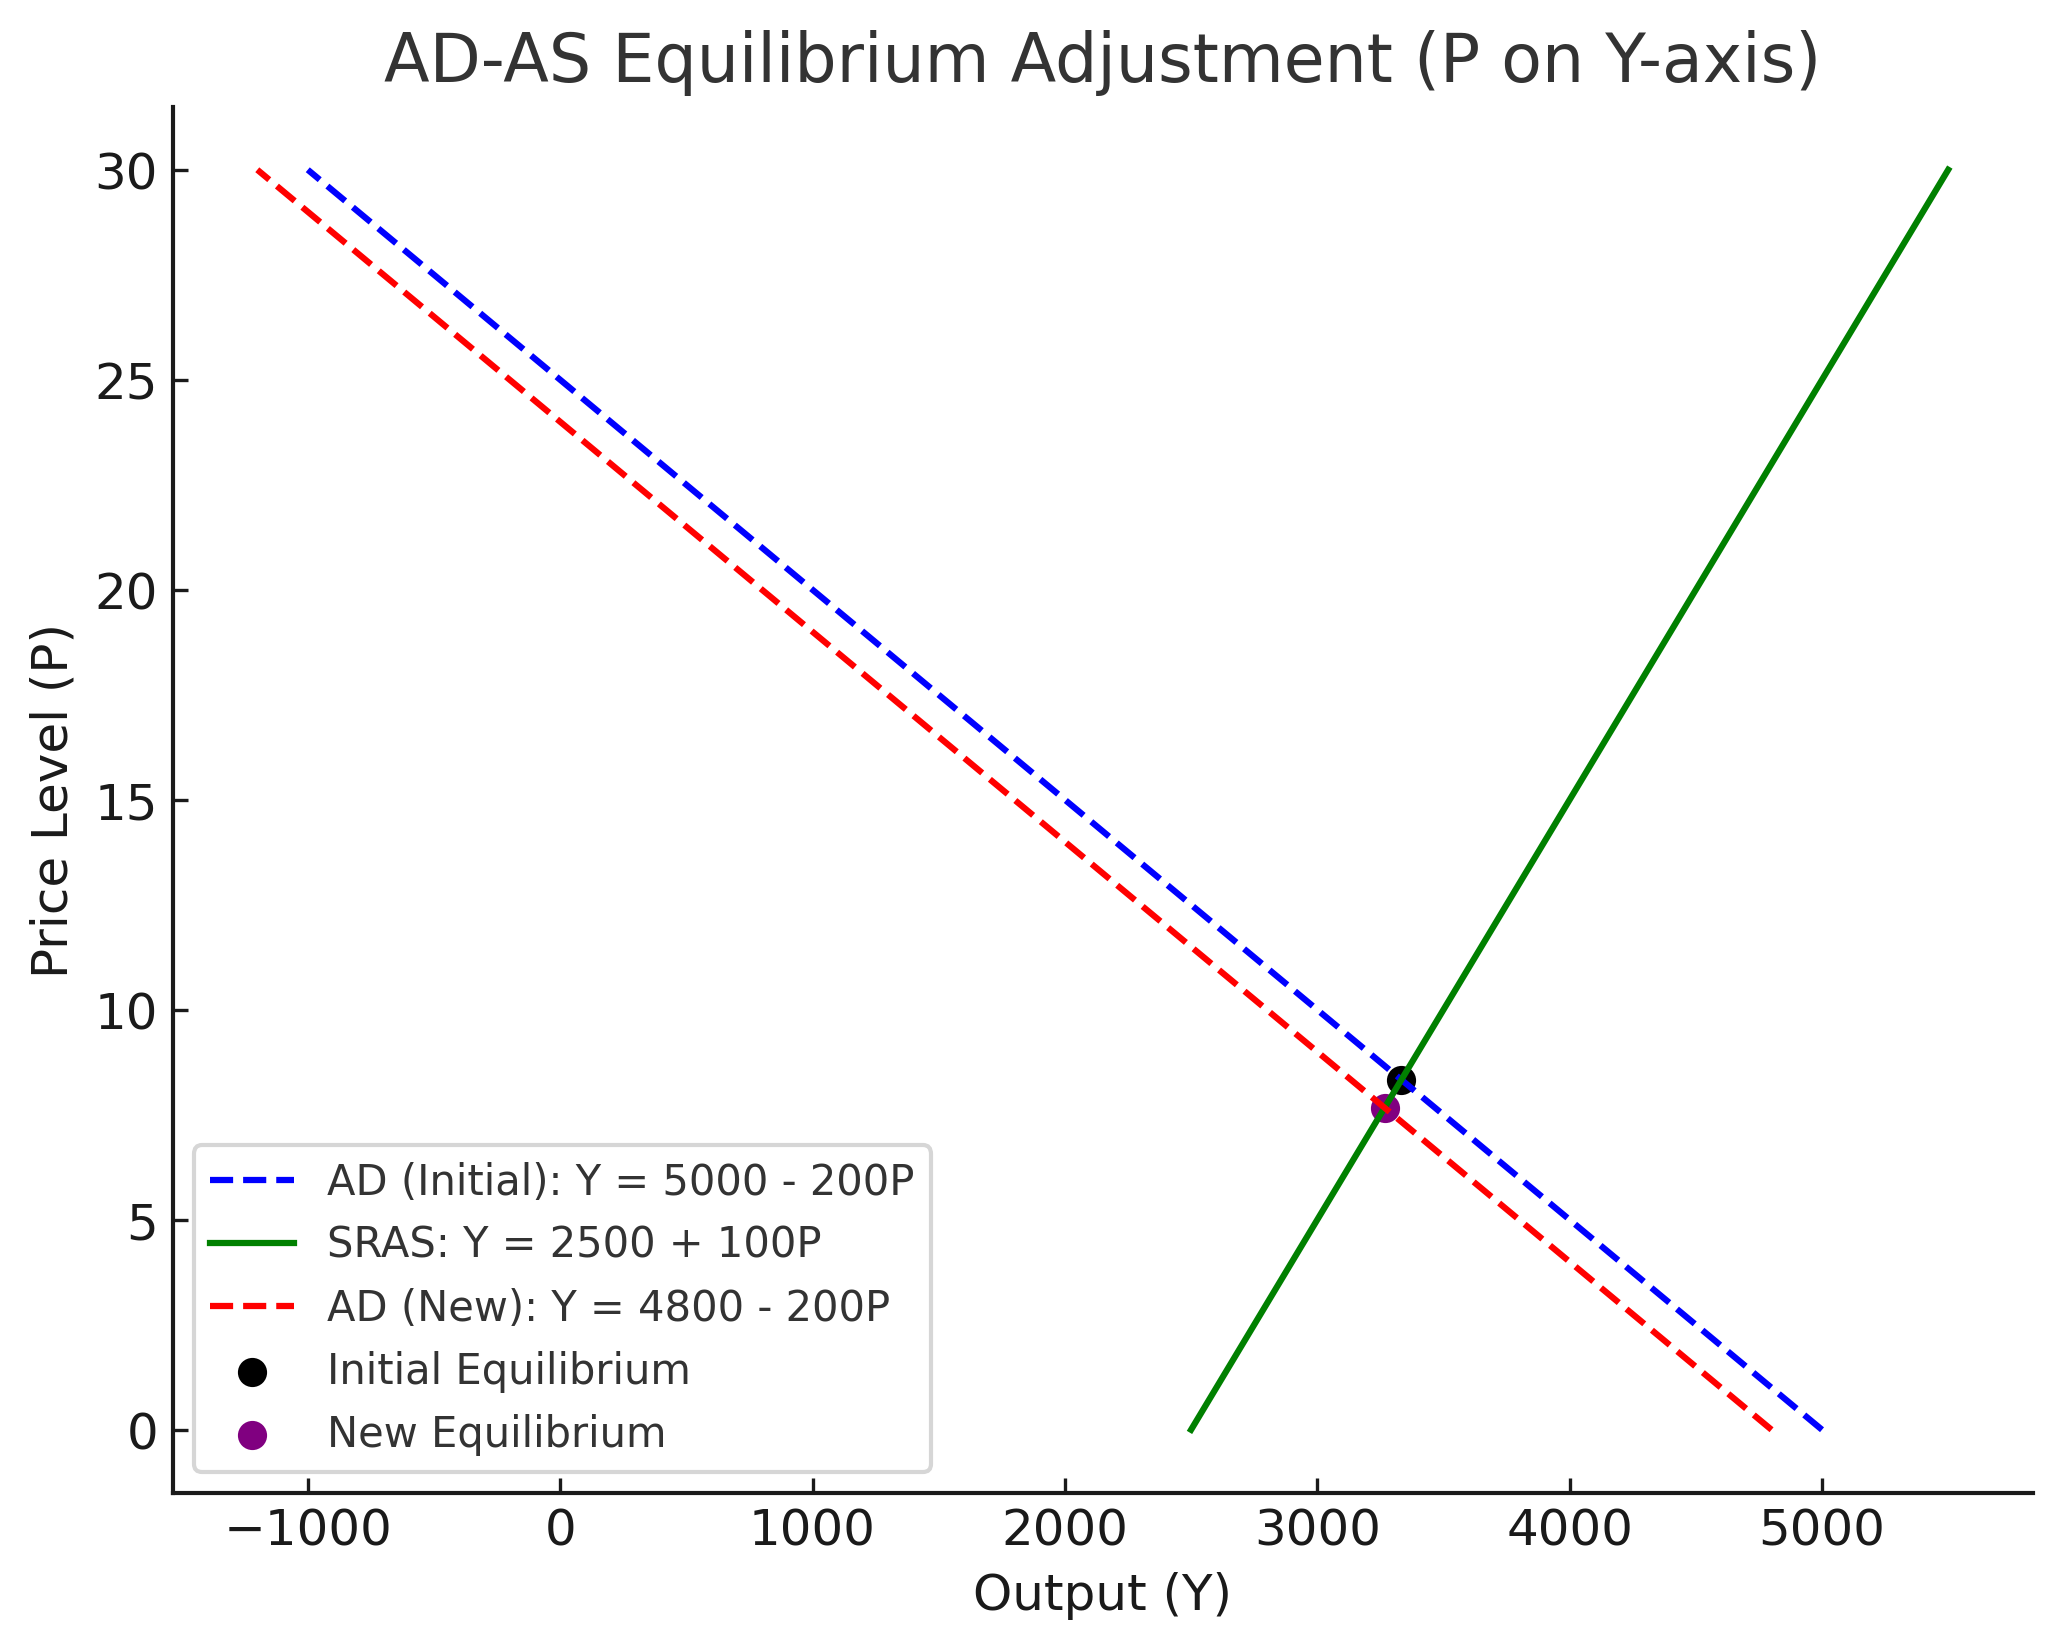
\includegraphics[width=0.7\textwidth]{PQ4_EX1.png}  % Insert your image file here
    
    \label{fig:sras_adjustment}
\end{figure}

\section*{Exercise 2: Graphing the Effects of a Negative Supply Shock}
Consider an economy in equilibrium at \(Y = 5500\) and \(P = 50\). A supply shock (e.g., an oil price increase) shifts SRAS leftward from:
\begin{align*}
    SRAS_1: & \quad Y = 3000 + 50P \\
    SRAS_2: & \quad Y = 2800 + 50P
\end{align*}

\textbf{Solutions:}
\section*{Macroeconomics Problem: Equilibrium after Supply Shock}

\textbf{Given:}
\begin{itemize}
    \item Initial equilibrium: \( Y = 5500 \), \( P = 50 \)
    \item Initial SRAS (SRAS1): \( Y = 3000 + 50P \)
    \item New SRAS (SRAS2): \( Y = 2800 + 50P \)
    \item Aggregate Demand (AD): \( Y = 8000 - 50P \)
\end{itemize}

\section*{Determine the new equilibrium price level and output.}

We set the aggregate demand (AD) equal to the new short-run aggregate supply (SRAS2) curve:
\[
AD = SRAS2
\]
\[
8000 - 50P = 2800 + 50P
\]
Solving for \( P \):
\[
8000 - 2800 = 50P + 50P
\]
\[
5200 = 100P
\]
\[
P = \frac{5200}{100} = 52
\]

Now, substitute \( P = 52 \) into the AD curve to find \( Y \):
\[
Y = 8000 - 50(52) = 8000 - 2600 = 5400
\]
Thus, the new equilibrium price level is \( P = 52 \) and the new equilibrium output is \( Y = 5400 \).

\section*{llustrate the shift in SRAS using a graph.}

To illustrate the shift in SRAS:
\begin{itemize}
    \item Initially, SRAS1 is \( Y = 3000 + 50P \), and the economy is at \( Y = 5500 \) and \( P = 50 \).
    \item After the supply shock, the new SRAS curve is \( Y = 2800 + 50P \).
    \item The AD curve is \( Y = 8000 - 50P \).
\end{itemize}
The AD curve remains unchanged, and the SRAS curve shifts leftward from SRAS1 to SRAS2, reflecting a decrease in output at each price level. The new equilibrium occurs at \( P = 52 \) and \( Y = 5400 \).

\begin{figure}[h!]
    \centering
    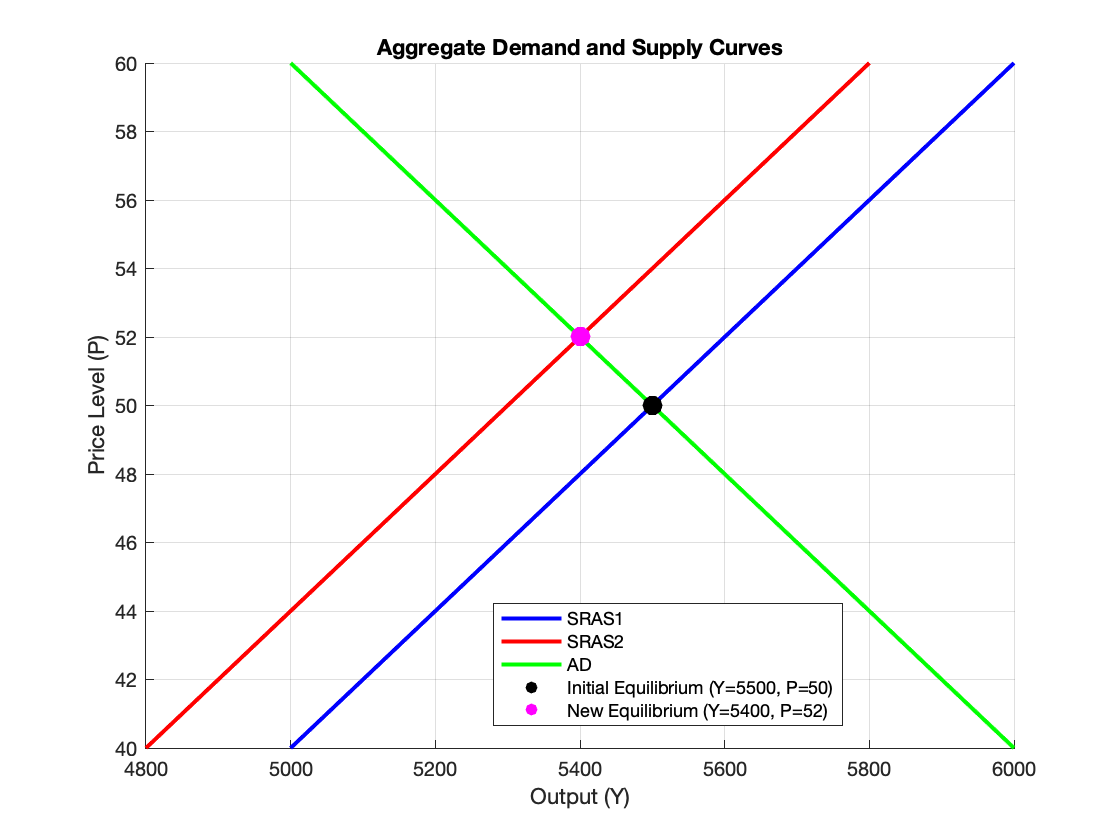
\includegraphics[width=0.7\textwidth]{PQ4_EX2.png}  % Insert your image file here
    
    \label{fig:sras_adjustment}
\end{figure}

\section*{What happens to inflation and unemployment after this shock?}

\begin{itemize}
    \item \textbf{Inflation:} The price level rises from \( P = 50 \) to \( P = 52 \), indicating an increase in inflation as the supply shock (e.g., oil price increase) pushes up costs, leading to higher prices.
    \item \textbf{Unemployment:} Output decreases from \( Y = 5500 \) to \( Y = 5400 \), implying a decline in economic activity, which leads to higher unemployment as firms reduce production and need fewer workers.
\end{itemize}

\section*{If the central bank responds by increasing the money supply, how would AD shift?}

If the central bank increases the money supply, the AD curve would shift to the right. This shift occurs because:
\begin{itemize}
    \item An increase in the money supply lowers interest rates, which stimulates investment and consumption.
    \item As a result, demand for goods and services increases, shifting the AD curve to the right.
    \item This would raise output and potentially increase the price level, helping to offset the negative impact of the supply shock on the economy.
\end{itemize}

\section*{Exercise 3: Fiscal Policy and AD Shifts}
Suppose the government implements an expansionary fiscal policy by increasing spending by \$200 billion. The marginal propensity to consume (MPC) is 0.8.

\textbf{Solutions:}
\begin{enumerate}
    \item Compute spending multiplier:
    \begin{align*}
        \text{Multiplier} &= \frac{1}{1 - 0.8} = 5
    \end{align*}
    \item Compute total GDP increase:
    \begin{align*}
        \Delta Y &= 5 \times 200 = 1000
    \end{align*}
    \item New AD equation: \( Y = 5000 - 100P \)
\end{enumerate}

\begin{figure}[h!]
    \centering
    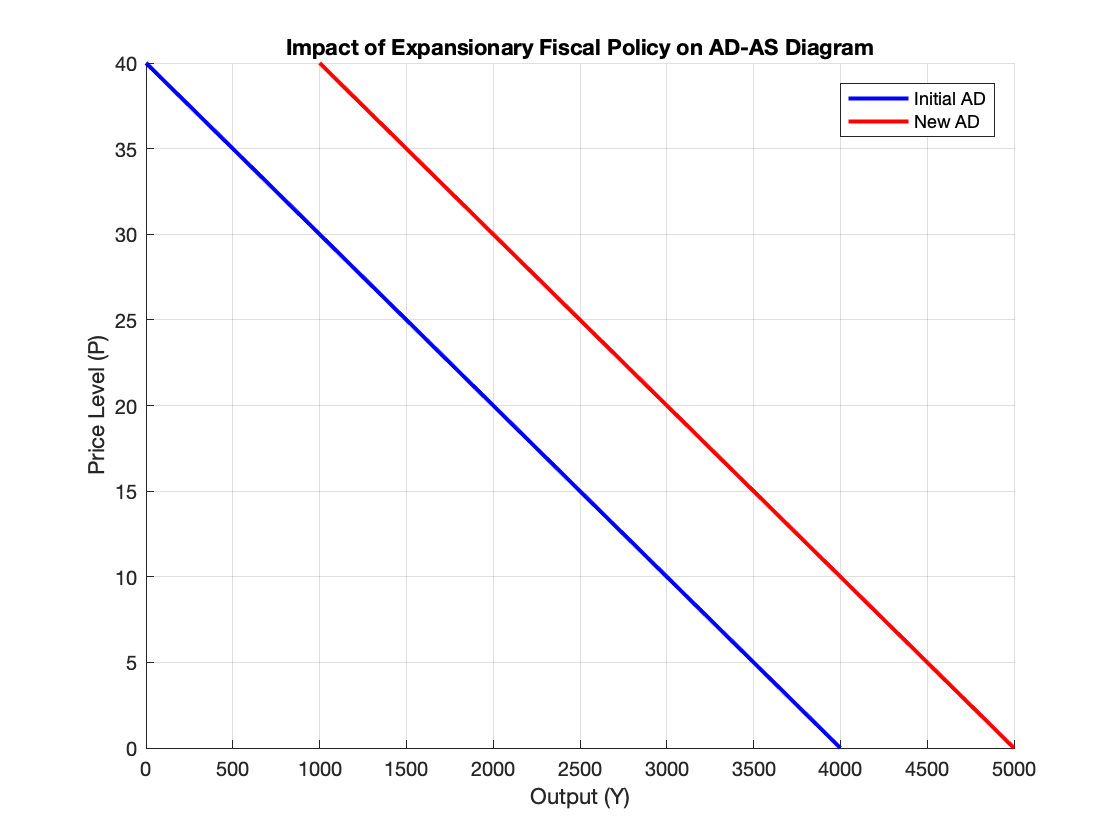
\includegraphics[width=0.7\textwidth]{PQ4_EX3.png}  % Insert your image file here
    
    \label{fig:sras_adjustment}
\end{figure}

\section*{Exercise 4: Long-Run Adjustment to a Recession}
An economy is experiencing a \textbf{recessionary gap} with actual GDP at \(2700\) and full-employment GDP at \(3000\). Assume wages are \textbf{sticky in the short run} but adjust over time.

\textbf{Solutions:}
\begin{enumerate}
    \item Graph the initial gap.
    \item Over time, SRAS shifts right as wages adjust.
    \item Government intervention can speed up recovery via fiscal/monetary policy.
    \item Classical economists advocate for self-correction, Keynesians favor active policy.
\end{enumerate}

\end{document}
